\scanpage{143}
% archive foliation: 142
% The typescript is upside down in the supplied scan; reading order follows the letter.
INSTITUT

DES HAUTES ÉTUDES SCIENTIFIQUES

91 - BURES-SUR-YVETTE

928-48-53

Massy November 21, 1966

Dear Mr Benjamin,

I got the front matter for the book ``Huit exposés ... '', which I am now sending back to you with two minor corrections. A more serious matter - and this is why I am adressing this letter to you rather than to Miss Ball - is the interrogation mark on page three concerning the mention ``Copyright 1966 by W.A. Benjamin, Inc ''. In your letter of july 8 1966, you stated that the copyright would remain with Mr Bourbaki, and I have been assuming till now that the book was being published under this proviso. If you should have changed your mind about it, I will have to check with Bourbaki if it is all right with him, which (whatever his decision) will cause a delay of a few months more. Once this matter set straight, everything is all right with me resp. the front matter, and you can go ahead$_x$ with the printing. I would only like to know if you got \unsure{my} letter of November 10 proposing to include still another paper, and your opinion about this suggestion.

Sincerely yours

\figure{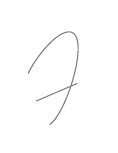
\begin{tikzpicture}[scale=.5]
\draw[gray] (0,0) .. controls (.45,.35) and (1,2.2) .. (.55,2.35) .. controls (.2,2.45) and (-.4,1.65) .. (-.55,1.3);
\draw[gray] (-.35,.6)--(.7,1.05);
\end{tikzpicture}}

